%!TEX program = xelatex
\documentclass[cn,hazy,blue,14pt,screen]{elegantnote}
\title{JapaneseNote:日本語勉強中}

\author{ティンバー・イエ}

\institute{Elegant\LaTeX{} Program}

% \version{2.30}
\date{\zhtoday}

%========================导言区==========================
\usepackage{array}
\usepackage{fontspec}
\usepackage{titletoc}
\usepackage{amssymb}
\usepackage{multicol} %用于实现在同一页中实现不同的分栏

\titlecontents{section}[0mm]
{\vspace{-2.2\baselineskip}\bfseries}
{\normalsize{\thecontentslabel}~\hspace{.5em}} {}
{\dotfill\contentspage[{\makebox[0pt][r]{\thecontentspage}}]}
[\vspace{-1.1\baselineskip}]
\dottedcontents{section}[1.16cm]{\large}{1.0em}{4pt}
\dottedcontents{subsection}[2.00cm]{\normalsize}{2.0em}{4pt}

\newcommand{\I}{\uppercase\expandafter{\romannumeral1}}
\newcommand{\II}{\uppercase\expandafter{\romannumeral2}}
\newcommand{\III}{\uppercase\expandafter{\romannumeral3}}
%========================导言区==========================

\begin{document}

\maketitle

\vspace{.8in}
\centerline{
  
\includegraphics[width=0.2\textwidth]{logo-blue.png}
}

\newpage
\tableofcontents

\newpage
\setcounter{page}{1}

%==============正文==================
\section{动词活用形}

\addcontentsline{toc}{subsection}{动词的种类}
\subsection*{动词的种类}

日语的句子结构是列举一堆体言,每一个都用助词修饰表示它在句子里的成分,然后一个用言结束句子表达整个句子的含义。更正确的讲,用言是可以活用的词(动词, 形容词 \, etc),活用是指通过变形表达时态否定,使役,被动等等。体言则没有活用(名词,数词etc)。

本讲介绍这些活用形是如何变化的,在实际上是如何构成了各种活用形,举例来说明其特点。每部分首先讲述如何变换,然后讲其实际应用。动词由原形(字典形)变成各种活用形时,\I 类动词(也叫五段动词)、\II 类动词(也叫一段动词)、\III 类动词(即サ变动词、カ变动词)的变化规律是不一样的。因此,看见动词,首先要学会辨别{\bfseries 动词的种类}。

\begin{itemize}
    \item {\bfseries \I 类动词} 指以除る以外的其他う段假名接尾的动词; 以る接尾,る前的假名不在い段或者え段上。
    
    如:買う(かう)、喜ぶ(よろこぶ)、行く(いく)、飲む(のむ)、勝つ(かつ)、倒す(たおす)、知る(しる)、作る(つくる)、分かる(わかる)等等。

    以下特殊词语(以る接尾,る前的假名在い段或者え段上,但为{\I 类动词}):焦る(あせる)、要る(いる)、煎る(いる)、帰る(かえる)、返る(かえる)、限る(かぎる)、切る(切る)、覆る(くつがえる)、蹴る(ける)、遮る(さえぎる)、茂る(しげる)、湿る(しめる)、知る(しる)、滑る(すべる)、散る(ちる)、照る(てる)、握る(にぎる)、練る(ねる)、罵る(ののしる)、入る(はいる)、走る(はしる)、減る(へる)、参る(まいる)、混じる(まじる)、漲る(みなぎる)。
    \vspace{0.2in}
    \item {\bfseries \II 类动词} 指词尾为る,倒数第二个假名为い段或者え段。
    
    例:見る(みる)、食べる(たべる)、考える(かんがえる)、助ける(たすける)、別れる(わかれる)等。
    \vspace{0.2in}
    \item {\bfseries \III 类动词} 又叫サ変动词、カ変动词。サ変动词主要是指する/词干+する(例:洗濯する(せんたくする)、掃除する(そうじする)、勉強する(べんきょうする))的词汇,カ変动词是指动词来る(くる)。
    
\end{itemize}

\subsection{未然形}

\subsubsection{变化规则}
\begin{itemize}
    \item {\bfseries \I 类动词} 动词词尾变成其所在行的あ段字,如果词尾是う则需要变成わ。
    
    例如:
    \begin{multicols}{2}
        \begin{enumerate}
            \item 読む(よむ)$\longrightarrow$読ま(よま)
            \item 買う(かう)$\longrightarrow$買わ(かわ)
            \item 書く(かく)$\longrightarrow$書か(かか)
            \item 死ぬ(しぬ)$\longrightarrow$死な(しな)
            \item 呼ぶ(よぶ)$\longrightarrow$呼ば(よば)
            \item 上がる(あがる)$\longrightarrow$上がら(あがら)
            \item 切る(きる)$\longrightarrow$切ら(きら)
            \item 帰る(かえる)$\longrightarrow$帰ら(かえら)
            \item 倒す(たおす)$\longrightarrow$倒さ(たおさ)
            \item 殴る(なぐる)$\longrightarrow$殴ら(なぐら)
        \end{enumerate}

    \end{multicols}

    \item {\bfseries \II 类动词} 去掉动词词尾中的る
    
    例如:
    \begin{multicols}{2}
        \begin{enumerate}
            \item 見る(みる)$\longrightarrow$見(み)
            \item 食べる(たべる)$\longrightarrow$食べ(たべ)
            \item 考える(かんがえる)$\longrightarrow$考え(かんがえ)
            \item 助ける(たすける)$\longrightarrow$助け(たすけ)
            \item 別れる(わかれる)$\longrightarrow$別れ(わかれ)
            \item 起きる(おきる)$\longrightarrow$起き(おき)
        \end{enumerate}

    \end{multicols}


    \item {\bfseries \III 类动词} {\texttt{サ变动词}}:根据不同的需要,する分别变成し、さ、せ。\texttt{カ变动词}:くる变成こ。
    
    例如:
    \begin{multicols}{2}
        \begin{enumerate}
            \item する$\longrightarrow$し、さ、せ
            \item 勉強する$\longrightarrow$勉強し、勉強さ、勉強せ
            \item 来る(くる)$\longrightarrow$こ
        \end{enumerate}

    \end{multicols}
    
\end{itemize}

\subsubsection{各种实用例}

\begin{enumerate}[A]
    \item {\bfseries 否定}:未然形+ない
        \begin{itemize}
            \item {\jp 私は本を{\bfseries 読まない}。}(我不读书。)
            \item {\jp 田中さんは晩御飯を{\bfseries 食べなかった}。}(田中没有吃晚饭。)
            \item {\jp 今日は日曜日だから、山田さんは{\bfseries 来ない}。}(今天是星期日,所以山田不来。)
        \end{itemize}
        \vspace{0.2in}
    \item {\bfseries 被动(被动态)}:{\uppercase\expandafter{\romannumeral1} 类动词未然形$+$れる、\uppercase\expandafter{\romannumeral2} 类动词未然形$+$られる、\uppercase\expandafter{\romannumeral3} 类动词({\texttt{サ变动词}}さ未然形$+$れる,\texttt{カ变动词}未然形+られる)}
        \begin{itemize}
            \item {\jp 弟は兄に{\bfseries 殴られた}。}(弟弟被哥哥打了。)
            \item {\jp 授業中話をして先生に{\bfseries 注意された}。}(上课说话,被老师批评了。)
            \item {\jp 大学の友達に{\bfseries 来られて}出られなくなりました}(大学里的朋友来了,不能出去了。)
            \item {\jp 私は弟にカメラを{\bfseries 壊されました}。}(我的相机被弟弟弄坏了。)
            \item {\jp この歌はいろいろな国で{\bfseries 歌われています}。}(这首歌在许多国家都唱。)
        \end{itemize}
        \vspace{0.2in}
    \item {\bfseries 可能(能动态)} \uppercase\expandafter{\romannumeral1} 类动词能动态较被动态相比,发生了{\heiti 约音变},あ段和后面的れ结合, 即动词原型词尾,变え段音+る。\uppercase\expandafter{\romannumeral2} 类动词可能态较被动态相比,完全一致,即未然形+られる。{\texttt{サ变动词}}不再是される,而是直接将する变成できる,\texttt{カ变动词}依然是 未然形+られる。
    \begin{itemize} 
        \item {\jp 眠くて、朝早く{\bfseries 起きられない}。}(太困了,早晨不能起早。)
        \item {\jp 道路(どうろ)が渋滞(じゅうたい)で早く{\bfseries 来られない}。}(道路拥挤,不能早来。)
        \item {\jp 私はまだ日本語で手纸が{\bfseries 書けません}。}(我还不会用日语写信。)
        \item {\jp 彼は今日本語の小说が{\bfseries 読める}ようになった。}(他现在好像能读懂日语小说了。)
    \end{itemize}
        \vspace{0.2in}
    \item {\bfseries 敬语助动词(变化同被动态)}:{\uppercase\expandafter{\romannumeral1} 类动词未然形$+$れる、\uppercase\expandafter{\romannumeral2} 类动词未然形$+$られる、\uppercase\expandafter{\romannumeral3} 类动词({\texttt{サ变动词}}さ未然形$+$れる,\texttt{カ变动词}未然形+られる)}
    \begin{itemize}
        \item {\jp 小林先生はいつもお宅で新聞を{\bfseries 読まれます}。}(小林先生总是在家读报纸。)
        \item {\jp 佐藤先生は学校まで遠いので、朝早く{\bfseries 起きられます}。}(佐藤先生家离学校很远,所以每天早晨很早起床。)
        \item {\jp 社長は会議に{\bfseries 参加されました}。}(总经理参加了会议。)
        \item {\jp 今朝部長はとても早く{\bfseries 来られました}。}(今天早晨部长来得很早。)
    \end{itemize}        
    \vspace{0.2in}
    \item {\bfseries 使役(使役态)}:{\uppercase\expandafter{\romannumeral1} 类动词未然形$+$せる、\uppercase\expandafter{\romannumeral2} 类动词未然形$+$させる、\uppercase\expandafter{\romannumeral3}类动词({\texttt{サ变动词}}さ未然形$+$せる,\texttt{カ变动词}未然形+させる)}
    \begin{itemize}
        \item {\jp 息子をイギリスへ{\bfseries 留学させます}。}(我让儿子去英国留学。)
        \item {\jp 私は娘を自由に{\bfseries 遊ばせました}。}(我让我女儿自由地玩耍。)
        \item {\jp 私は息子に道路の右側を{\bfseries 歩かせます}。}(我让孩子在道路的右侧走路。)
        \item {\jp 先生は学生に自由に意見を{\bfseries 言わせました}。}(老师让学生自由地发表意见。)
    \end{itemize}
    
    \vspace{0.2in}
    \item {\bfseries 被役(被役态)}:被役态的变形规律是 先将动词变成使役态,再变成被动态。
    
    \uppercase\expandafter{\romannumeral1} 类动词未然形$+$せる$+$られる$\longrightarrow$约音\footnote{原形是以す结尾时,则不发生约音。}, 动词未然形$+$される。

    \uppercase\expandafter{\romannumeral2} 类动词未然形$+$させる$+$られる$\longrightarrow$动词未然形$+$させられる。

    \uppercase\expandafter{\romannumeral3} 类动词未然形$+$させる$+$られる$\longrightarrow$动词未然形$+$させられる。

        \begin{itemize}
            \item {\jp 行きたくないのですが、母に病院へ{\bfseries 行かされました}}(我不想去,但是被母亲逼着,去了医院。)
            \item {\jp 子供の時は食べたくない物を沢山{\bfseries 食べさせられました}。}(小时候,有很多不想吃的东西,都被逼着吃了。)
            \item {\jp 毎日学校に{\bfseries 来させられます}が、自分でも何をしているか分かりません。}(每天被逼着上学,但是连自己都不知道在干什么。)
        \end{itemize}
    
    \vspace{0.2in}
    \item {\bfseries 否定推量和否定意志(\uppercase\expandafter{\romannumeral1} 类动词除外)}:未然形+まい
    
    \begin{itemize}
        \item {\jp こんな酸っぱい果物は二度と{\bfseries 食べまい}。}(这样酸的水果,我再也不吃了。)
        \item {\jp 天気が悪いから、浅田さんは{\bfseries 来まい}。}(因为天气不好,所以浅田先生不会来了。)
    \end{itemize}

    \vspace{0.2in}
\end{enumerate}


\subsection{连用形}
在实际使用中,连用形是使用频率最高的活用形。

\subsubsection{变化规则}

\begin{itemize}
    \item {\bfseries \I 类动词}\, 连用形有2种:
    
    {\bfseries 连用形 1}的词尾是该行的い段假名:
    \begin{multicols}{2}
        \begin{enumerate}
            \item 読む(よむ)$\longrightarrow$読み(よみ)
            \item 買う(かう)$\longrightarrow$買い(かい)
            \item 書く(かく)$\longrightarrow$書き(かき)
            \item 死ぬ(しぬ)$\longrightarrow$死に(しに)
            \item 呼ぶ(よぶ)$\longrightarrow$呼び(よび)
            \item 上がる(あがる)$\longrightarrow$上がり(あがり)
            \item 切る(きる)$\longrightarrow$切り(きり)
            \item 帰る(かえる)$\longrightarrow$帰り(かえり)
            \item 倒す(たおす)$\longrightarrow$倒し(たおし)
            \item 殴る(なぐる)$\longrightarrow$殴り(なぐり)
        \end{enumerate}

    \end{multicols}

    {\bfseries 连用形 2}又称作“五段动词连用形的音变浊化”,在「て、ては、ても、た、たら、たり」这6个助词或助动词前面使用.

    \begin{multicols}{2}
        \begin{enumerate}
            \item 書く(かく)$\longrightarrow$書いた、書いて
            \item 泳ぐ(およぐ)$\longrightarrow$泳いだ、泳いで $\blacksquare$ 

            \item 読む(よむ)$\longrightarrow$読んだ、読んで
            \item 学ぶ(まなぶ)学んだ、学んで
            \item 呼ぶ(よぶ)$\longrightarrow$呼んだ、呼んで
            \item 死ぬ(しぬ)$\longrightarrow$死んだ、死んで
            $\blacksquare$ 
            
            \item 買う(かう)$\longrightarrow$買い(かい)
            \item 待つ(まつ)待った、待って
            \item 上がる(あがる)$\longrightarrow$上がった、上がって
            \item 切る(きる)$\longrightarrow$切った、切って
            \item 帰る(かえる)$\longrightarrow$帰った、帰って
            $\blacksquare$ 
            
            \item 倒す(たおす)$\longrightarrow$倒した、倒して
            \item 騙す(だます)$\longrightarrow$騙した、騙して
            $\blacksquare$ 
            
            \item 行く$\longrightarrow$行った、行って
            $\blacksquare$     
        \end{enumerate}

    \end{multicols}
    
    \item {\bfseries \II 类动词}去掉动词词尾中的る(同未然形)。
    
    \begin{multicols}{2}
        \begin{enumerate}
            \item 見る(みる)$\longrightarrow$見(み)
            \item 食べる(たべる)$\longrightarrow$食べ(たべ)
            \item 考える(かんがえる)$\longrightarrow$考え(かんがえ)
            \item 助ける(たすける)$\longrightarrow$助け(たすけ)
            \item 別れる(わかれる)$\longrightarrow$別れ(わかれ)
            \item 起きる(おきる)$\longrightarrow$起き(おき)
        \end{enumerate}

    \end{multicols}

    \item {\bfseries \III 类动词}
    
    サ变动词:する变成し。 勉強する$\longrightarrow$勉強し

    カ变动词:来る$\longrightarrow$き

    

\end{itemize}

\subsubsection{各种实用例}

\begin{enumerate}[A]
    \item 连用法
    \begin{enumerate}[a]
        \item 连用形+始まる、続ける、終わる、出す、過ぎる、残す、返す、込む、かける、合う、切る、かねる、得る等构成{\bfseries 复合动词}。
        \begin{itemize}
            \item {\jp {\bfseries 読みかけた}本のページに印(しるし)をつける。}(在读了一部分的书页上作记号。动词连用形+かける表示动作还没结束)
            \item {\jp {\bfseries 勉強し続ける}ためには健康な体が必要です。}(为了继续学习,需要健康的身体。)
            \item {\jp {\bfseries 食べ終わったら}片づけてください。}(吃完了后给收拾一下。)
            \item {\jp これは昼食{\bfseries 食べ残した}料理だ。}(这是午饭吃剩下的菜。)
            \item {\jp {\bfseries 食べ過ぎ}て、お腹がいっぱいです。}(吃得太多了,肚子饱饱的。)
            \item {\jp 物理学の研究に{\bfseries 打ち込む}。}(热衷于物理研究。)
            \item {\jp 彼女は旅行に行くかどうか{\bfseries 決めかねている}。}(她难下决定是否要去旅行。)
            \item {\jp {\bfseries 付き合って}ください!}(请和我交往吧!)
            \item {\jp 二人で冷蔵庫にあるビールを全部{\bfseries 飲み切って}しまった。}(两个人把冰箱里的啤酒喝了个精光。)
            \item {\jp 別に君をまた好きになることなんて{\bfseries ありえない}けど、君のドルチェ&ガッバーナの香水が思い出させる。}
        \end{itemize} 
        \item 连用形+やすい、にくい等来构成复合形容词。
        \begin{itemize}
            \item {\jp この万年筆は{\bfseries 書きやすい}です。}(这只钢笔很好写。)
            \item {\jp この服はとても格好(かっこう)がいいが、非常(ひじょう)に{\bfseries 着にくい}。}(这一部分是很容易掌握的内容。)
            \item {\jp この部分は{\bfseries 把握し(はあく)やすい}内容(ないよう)だ。}(这一部分是很容易掌握的内容。)
            \item {\jp ここはなかなか{\bfseries 来にくい}場所である。}(这里是很不容易来的地方。)
        \end{itemize}

        \item 动词连用形2+て+(狭义的)补助动词\href{https://www.zhihu.com/question/433110548/answer/1609376134}{てくる、ていく、ている、てある、てみる、ておく}。
        \begin{itemize}
            \item {\jp 学校へお弁当を{\bfseries 持っていく}。}(带着便当去学校。)
            \item {\jp たくさんの人が{\bfseries 乗ってくる}。}(许多人上车了。)
            \item {\jp 兄は今本を{\bfseries 読んでいます}。}(哥哥现在正在读书。)
            \item {\jp 窓が{\bfseries 開けてあります}}(窗户开着。)
            \item {\jp 今まで日本語を{\bfseries 勉強してきた}。}(一直学日语到现在。)
            \item {\jp ちょっとジュースを{\bfseries 買ってくる}。}(我去买个饮料回来。)
            \item {\jp 友達が来るから、部屋を{\bfseries 掃除しておき}ました。}(因为朋友要来,所以我把房间收拾干净了。)
            \item {\jp ここへ{\bfseries 来てみて}はじめてここの立派(りっぱ)さに驚(おどろ)いた。}(来到这里,才知道这里的壮观程度。)
            \item {\jp 買ったばかりの傘をどこかに{\bfseries 忘れてきてしまった}。}(刚买的伞忘了放在哪里了。)
            \item {\jp この宿題を{\bfseries してしまったら}、ゲームで遊ぼう。}(把这项作业做完之后,来打电玩吧!)
        \end{itemize}

        \item 连用形+名词构成复合名词。
        \begin{multicols}{2}
            \begin{enumerate}[1.]
                \item 買い物
                \item 贈り物
                \item 読み方
                \item 寝言(ねごと)
                \item 足し算(たしざん)
                \item 飲み物
                \item 忘れ物
            \end{enumerate}
    
        \end{multicols}

    \end{enumerate}

    \item 中顿法
    \begin{enumerate}[a]
        \item 用于连接2个单句,使之变成一个并列句。
        \begin{itemize}
            \item {\jp 雨が{\bfseries 降り}、風も吹いている。}(又下雨,又刮风。)
            \item {\jp ご飯も{\bfseries 食べ}、御酒も飲みます。}(又吃饭,又喝酒。)
            \item {\jp 日本語の勉強も{\bfseries し}、コンピュータの勉強もする。}(又学日语,又学计算机。)
        \end{itemize}
        \item 用于连接2个单句,使之表示2个连续的动作。
        \begin{itemize}
            \item {\jp 朝起きて、歯を{\bfseries 磨き}、顔を洗った。}(早晨起床后,刷牙、洗脸。)
            \item {\jp ご飯を{\bfseries 食べ}、お茶を飲んだ。}(吃饭(后)喝茶。)
            \item {\jp ラジオ体操を{\bfseries し}、ジョキングをした。}(作广播操,再慢跑。)
        \end{itemize}
        \item 表示动作的状态\\原因。
        \begin{itemize}
            \item {\jp 傘を{\bfseries 持ち}、出て行きました。}(拿着伞出去了。)
            \item {\jp 見たい映画を{\bfseries 見}、満足しました。}(看了想看的电影,所以很满意。)
            \item {\jp 先生が説明を{\bfseries し}、皆は分かりました。}(因为老师进行了说明,所以大家都明白了。)
        \end{itemize}
        
    \end{enumerate}
\end{enumerate}
\subsection{终止形}

\subsection{连体形}

\subsection{假定形}

\subsection{命令形}

\subsection{推量形}






%==============正文==================

\section{协作人员招募}

招募 Elegant\LaTeX{} 的协作人员,没有工资。工作内容:翻译 Elegant\LaTeX{} 系列模板相关的文稿(中翻英),维护模板的 wiki(主要涉及 Markdown),如果有公众号文稿写作经历的话,也可以帮忙写微信稿。本公告长期有效。

目前 ElegantLaTeX 共有 4 名协作人员,分别是
\begin{itemize}
  \item 官方文档翻译: \href{https://github.com/peggy2006xzyz}{YPY};
  \item GitHub 维基维护: \href{https://github.com/izinngo}{Ingo Zinngo}、\href{https://github.com/xiaohao890809}{追寻原风景};
  \item QQ 群管理员: \href{https://github.com/sikouhjw}{Sikouhjw}.
\end{itemize}

在此感谢他们无私的奉献!


\section{致谢}

截止到 2020 年 04 月 12 日,ElegantNote 2.30 版本发布,ElegantNote 模板在 GitHub 上的收藏数(star)达到了 263。在此特别感谢 China\TeX{} 以及 \href{http://www.latexstudio.net/}{\LaTeX{} 工作室}对于本系列模板的大力宣传与推广。如果你喜欢我们的模板,你可以在 GitHub 上收藏(Star)我们的模板。

\begin{figure}[htbp]
  \centering
  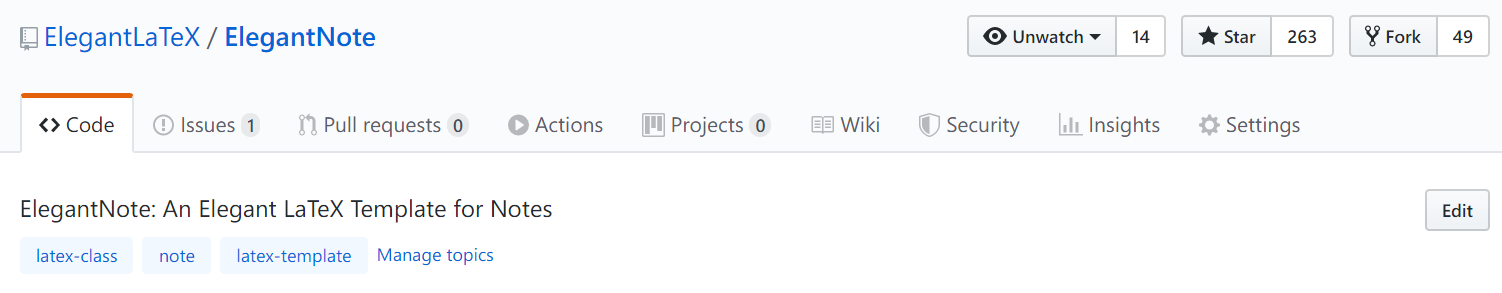
\includegraphics[width=\textwidth]{star.png}
  \caption{一键三连求赞}
\end{figure}


\section{捐赠}

如果您非常喜爱我们的模板,你还可以选择捐赠以表达您对我们模板和我的支持!

\begin{figure}[htbp]
  \centering
  
\includegraphics[width=0.4\textwidth]{donate.jpg}
\end{figure}

\textbf{赞赏费用的使用解释权归 Elegant\LaTeX{} 所有,并且不接受监督,请自愿理性打赏}。10 元以上的赞赏,我们将列入捐赠榜,并且发放捐赠纪念证(全部),谢谢各位金主!

\begin{table}[htbp]
  \scriptsize
  \centering
  \caption{Elegant\LaTeX{} 系列模板捐赠榜}
    \begin{tabular}{*{8}{>{\scriptsize}c}}
    \toprule
    \textbf{捐赠者} & \textbf{金额} & \textbf{时间} & \textbf{渠道} & \textbf{捐赠者} & \textbf{金额} & \textbf{时间} & \textbf{渠道} \\
    \midrule
    Lerh  & 10 RMB & 2019/05/15 & 微信    & 越过地平线 & 10 RMB & 2019/05/15 & 微信 \\
    银桑    & 20 RMB & 2019/05/27 & 微信    & *空    & 10 RMB & 2019/05/30 & 微信 \\
    latexstudio.net & 666 RMB & 2019/06/05 & 支付宝   & A*n   & 40 RMB & 2019/06/15 & 微信 \\
    * 夏   & 22 RMB & 2019/06/15 & 微信    & * 倩   & 21 RMB  & 2019/06/15 & 微信 \\
    Cassis & 11 RMB & 2019/06/30 & 微信    & *君    & 10 RMB & 2019/07/23 & 微信 \\
    P*u   & 50 RMB & 2019/07/30 & 微信    & *萌    & 19 RMB & 2019/08/28 & 微信 \\
    曲豆豆   & 10 RMB & 2019/08/28 & 微信    & 李博    & 100 RMB & 2019/10/06 & 微信 \\
    Njustsll & 10 RMB & 2019/10/11 & 微信    & 刘志阔   & 99.99 RMB & 2019/10/15 & 支付宝 \\
    * 韬   & 16 RMB & 2019/10/17 & 微信    & 赤霓    & 12 RMB & 2019/10/17 & 支付宝 \\
    追寻原风景 & 10 RMB & 2019/10/28 & 微信    & 郭德良   & 88 RMB & 2019/11/03 & 微信 \\
    自强不息  & 20 RMB & 2019/11/04 & 支付宝   & 读书之虫  & 20 RMB & 2019/11/18 & 微信 \\
    *等    & 10 RMB & 2019/11/18 & 微信    & *哲    & 20 RMB & 2019/11/18 & 微信 \\
    佚名    & 10 RMB & 2019/11/24 & 微信    & Jiye Qian & 66 RMB & 2019/12/04 & 微信 \\
    * 阳   & 20 RMB & 2019/12/05 & 微信    & Catcher & 11 RMB & 2019/12/08 & 支付宝 \\
    希尔波特门徒 & 10 RMB & 2019/12/09 & 支付宝   & * 伟   & 10 RMB & 2019/12/09 & 微信 \\
    Simon & 20 RMB & 2019/12/11 & 支付宝   & 流殇丶浅忆 & 66.60 RMB & 2019/12/18 & 支付宝 \\
    羽     & 10 RMB & 2019/12/20 & 支付宝   & * 琛   & 15 RMB & 2019/12/20 & 微信 \\
    随风    & 20 RMB & 2019/12/27 & 支付宝   & Ws    & 23.30 RMB & 2019/12/28 & 微信 \\
    初八    & 100 RMB  & 2020/01/02 & 支付宝   & p*e   & 20 RMB & 2020/01/03 & 微信 \\
    Shunmx & 100 RMB & 2020/01/03 & 微信    & hj    & 10 RMB & 2020/01/03 & 微信 \\
    F*5   & 10 RMB & 2020/01/03 & 微信    & S*m   & 20.20 RMB & 2020/01/03 & 微信 \\
    二代青雉  & 13 RMB & 2020/01/14 & 支付宝   & *?    & 66 RMB & 2020/01/15 & 微信 \\
    Mr. Xiong & 20 RMB & 2020/01/17 & 微信    & *博    & 15 RMB & 2020/01/18 & 微信 \\
    * 者  & 10 RMB & 2020/02/02 & 微信    & Jackie  &  88.80 RMB  &  2020/02/09 & 微信 \\
    Henry\_Sun、 & 50 RMB & 2020/02/14 & 支付宝 & * 桥  & 50 RMB & 2020/02/21 & 微信 \\
    昀琏 & 10 RMB & 2020/03/02 & 支付宝 & S*y  &  10 RMB  &  2020/03/15 & 微信 \\
    * 哥  & 66.66 RMB & 2020/03/17 & 微信    &   K*e & 30 RMB & 2020/03/30 & 微信\\
    * 阳  &  20 RMB  &  2020/04/02 & 微信 & 士*n  & 30 RMB & 2020/04/11 & 微信 \\
    \bottomrule
    \end{tabular}%
  \label{tab:donation}%
\end{table}%


\section{常见问题 FAQ}

\begin{enumerate}[label=\arabic*).]
  \item \textit{如何删除版本信息?}\\
    导言区不写 \lstinline|\version{x.xx}| 即可。
  \item \textit{如何删除日期?}\\
    与版本 \lstinline{\version} 不同的是,导言区不写或注释 \lstinline{\date} 的话,仍然会打印出当日日期,原因是 \lstinline{\date} 有默认参数。如果不需要日期的话,日期可以留空即可,也即 \lstinline|\date{}|。
  \item \textit{如何获得中文日期?}\\
    为了获得中文日期,必须在中文模式下,使用 \lstinline|\date{\zhdate{2019/12/09}}|,如果需要当天的汉化日期,可以使用 \lstinline|\date{\zhtoday}|,这两个命令都来源于 \href{https://ctan.org/pkg/zhnumber}{\lstinline{zhnumber}} 宏包。
  \item \textit{如何添加多个作者?}\\
    在 \lstinline{\author} 里面使用 \lstinline{\and},作者单位可以用 \lstinline{\\} 换行。
    \begin{lstlisting}
      \author{author 1\\ org. 1 \and author 2 \\ org. 2 }
    \end{lstlisting}
\end{enumerate}

\end{document}
